\section{Mejora del algoritmo propuesto (poda de resultados)}
	\subsection{Descripción del algorítmo}

	Las podas apuntan a obviar el cálculo de soluciones que ya sabemos peores que otras ya calculadas:

	\begin{itemize}

		\item Si sabemos que en alguna rama encontramos una solución final de tamaño i y la rama actual tiene una solución parcial de $j \leq i$, podemos obviar el resto de la rama actual.

		\item Si sabemos que existe una rama con solución final 0, existe una solución óptima y no requerimos calcular nada más.

	\end{itemize}

	A continuación se propone un algoritmo para las llamadas recursivas. Para el caso inicial, se toma $Indice = 0$, $Actual = 0$ y $Mejor = |Lista|$.

	La variable $Mejor$ es de entrada/salida, es decir, las llamadas recursivas pueden modificar el valor. Al final del algoritmo, la misma almacenará el mejor resultado.

	\begin{algorithm}[H]
		\NoCaptionOfAlgo
		
		\KwData{Lista, la lista de números a pintar}

		\KwData{UltRojo, el valor del úlitmo rojo que pintamos}

		\KwData{UltAzul, el valor del úlitmo azul que pintamos}

		\KwData{Indice, la posición que estamos mirando ahora}

		\KwData{Actual, la cantidad de elemntos no pintados hasta ahora}

		\KwData{Mejor, la mejor solución hasta ahora}

		\If{Actual $<$ Mejor} {
			\uIf{Indice == $|Lista|$}{
				Llegamos al final de la lista

				Mejor es Actual
			}
			\Else{
				\If{no existe UltRojo \textbf{or} UltRojo $<$ Lista[Indice]}{
					Calcular el mejor resultado pintando de Rojo

					Llamada Recursiva: \{Lista, Lista[Indice], UltAzul, Indice+1, Res, Mejor\}

					La función modifica el valor de Mejor si corresponde
				}
				\If{Mejor $\neq$ 0}{
					\If{no existe UltAzul \textbf{or} UltAzul $>$ Lista[Indice]}{
						Calcular el mejor resultado pintando de Azul

						Llamada Recursiva: \{Lista, UltRojo, Lista[Indice], Indice+1, Res, Mejor\}

						La función modifica el valor de Mejor si corresponde
					}
					\If{Mejor $\neq$ 0}{
						Calcular el mejor resultado sin pintar

						Llamada Recursiva: \{Lista, UltRojo, UltAzul, Indice+1, Res+1, Mejor\}

						La función modifica el valor de Mejor si corresponde
					}
				}
			}
		}

		\KwResult{Ninguno, pero Mejor puede ser modificado si se encuentra una mejor subsolución.}
	\end{algorithm}

	A diferencia del algoritmo de Backtracking básico, el orden en que se calculan los casos recursivos es importante, ya que podemos encontrar un caso óptimo y podar el resto del espacio de soluciones.

	\pagebreak
	\subsection{Cota de complejidad}

	El algoritmo propuesto, al igual que el algorítmo base de Backtracking, realiza hasta tres llamadas recursivas en cada paso. En mejor caso, no se realiza ninguna llamada recursiva (se realiza una poda).

	En cualquier llamada recursiva, el tamaño del problema a resolver disminuye en 1 (se avanza/pinta un solo número).

	La función de complejidad sería
	\[
	T(BTMejorado(n)) =
		\begin{cases}
			\text{1,} &\quad\text{si n == 0}\\
			\text{3 T(BTMejorado(n-1)),} &\quad\text{si no} \\
		\end{cases}
	\]

	donde n es la cantidad de números restantes, es decir, $|Lista| - Indice$.

	Es decir, en órdenes de complejidad, BTMejorado (Backtracking con podas) es igual a BT (Backtracking sin podas).

	Esto no quiere decir que las podas son irrelevantes, las mismas pueden cortar el tiempo de procesamiento de manera importante, pero los cambios en complejidad son de orden menor a $3^n$, por lo que esta sigue siendo la complejidad en peor caso.

	El mejor caso para el algoritmo se da si la lista es estrictamente creciente. En este caso, se realiza solo una llamada recursiva por nivel, hallando un caso óptimo al llegar al final de la lista y podando el resto, por lo que la complejidad resultante es de $\Omega(n)$.

	Este es un detalle implementativo, ya que en el algoritmo propuesto primero se realizan las llamdadas recursivas pintando de rojo de ser posible. De haberse utilizado un orden distinto, el mejor caso podría haberse dado con una entrada diferente.

	\subsection{Gráfico de complejidad}

	El siguiente gráfico utiliza el mismo criterio que el anterior. Si bien la diferencia no es visualmente notoria, debe notarse que los valores del eje vertical son mucho menores (alrededor de 1/10 de los valores equivalentes sin poda).

	\begin{center}
	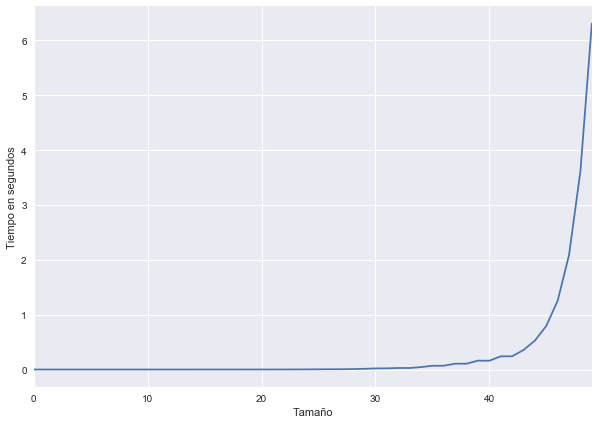
\includegraphics[width=.8\textwidth]{ej2.png}
	\end{center}

	Se agrega también el siguiente gráfico en el que se muestran ambos algoritmos, utilizando una escala logarítmica para poder comparar mejor los órdenes de complejidad. El algoritmo mejorado es irregular debido a que las listas testeadas son aleatorias y pueden tener mejor o peor comportamiento frente a las podas definidas.

	Como evidencia el gráfico logarítmico, si bien la mejora con las podas es notoria (como se mencionó antes, aproximadamente 1/10 del tiempo), ambos algorítmos crecen en órdenes similares.

	\begin{center}
	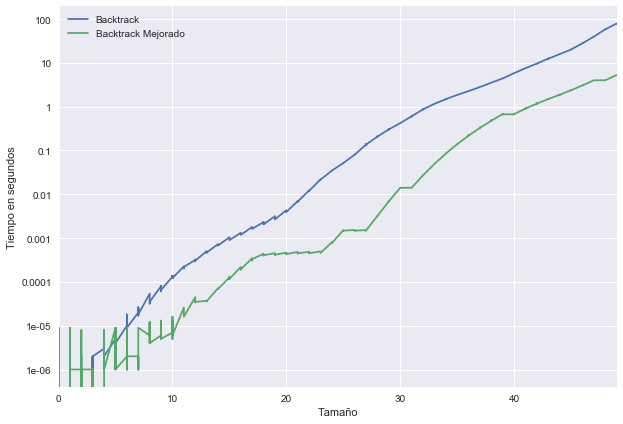
\includegraphics[width=.8\textwidth]{ej2-2.png}
	\end{center}

	Como nota final, al analizar el mejor caso del algoritmo, el tiempo de procesado de estas era casi despreciable ya que la complejidad es lineal al tamaño de la lista. Por este motivo, no es práctico comparar estos casos, pero si se incluye un gráfico ilustrativo de dicho caso, medido con listas de enteros consecutivos entre 1 y $|Lista|$. Notese que el tiempo está medido en nanosegundos por el requerimiento de precisión extrema, y las mediciones tienen ruido por procesamiento ajeno al problema.

	\begin{center}
	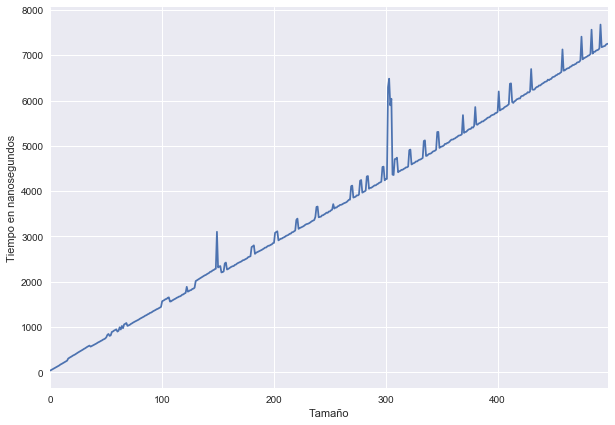
\includegraphics[width=.8\textwidth]{ej2-3.png}
	\end{center}